%!TEX root = main.tex

\section{Prioritized Streaming String Transducers}  \label{sect:psst}
%\zhilin{Move from preliminary to here}

In this section, we introduce prioritized streaming string transducers (PSST), 
a new class of transducers that combine prioritized finite-state automata \cite{BM17} 
and streaming string transducers \cite{AC10,AD11}.
We shall utilize PSSTs to model greedy/lazy semantics of Kleene star/plus as well as the behavior of the $\extract$ and $\replaceall$ functions.
%based on which we model the semantics of $\regexp$ defined in Section~\ref{sec:prel} and design the decision procedure in Section~\ref{sec:decision}.

%\paragraph{Prioritized Finite-state automata.}

\vspace{-1mm}
\begin{definition}[Finite-state Automata] \label{def:nfa}
	A \emph{(nondeterministic) finite-state automaton}
	(\FA{}) over a finite alphabet $\ialphabet$ is a tuple $\Aut =
	(\ialphabet, \controls, q_0, \finals, \transrel)$ where 
	$\controls$ is a finite set of 
	states, $q_0\in \controls$ is
	the initial state, $\finals\subseteq \controls$ is a set of final states, and 
	$\transrel\subseteq \controls \times 
	\ialphabet^\varepsilon \times  \controls$ is the
	transition relation. 
\end{definition}
\vspace{-1mm}

For an input string $w$, a \emph{run} of $\Aut$ on $w$
%(with $a_0 = \EndLeft$ and $a_{n+1} = \EndRight$)
is a sequence $q_0 a_1 q_1 \ldots a_n q_n$ such that $w = a_1 \cdots a_n$ and $(q_{j-1}, a_{j}, q_{j}) \in
\transrel$ for every $j \in [n]$.
The run is said to be \defn{accepting} if $q_n \in \finals$.
A string $w$ is \defn{accepted} by $\Aut$ if there is an accepting run of
$\Aut$ on $w$. 
%In particular, the empty string $\varepsilon$ is accepted by $\Aut$ if $q_0 \in F$. 
The set of strings accepted by $\Aut$, i.e., the language \defn{recognized} by $\Aut$, is denoted by $\Lang(\Aut)$.
%Since we deal with computational complexity in the sequel, we define
The \defn{size} $|\Aut|$ of $\Aut$ is defined as the cardinality of the set $Q$ of states.
%, which will be 
%used when the computational complexity is concerned.

%
For a finite set $Q$, let $\overline{Q} = \bigcup_{n\in \Nat}\{ (q_1, \ldots, q_n) \mid \forall i \in [n], q_i \in Q \wedge \forall i,j \in[n], i \neq j \rightarrow q_i \neq q_j \}$. Intuitively, $\overline{Q}$ is the set of sequences of non-repetitive elements from $Q$. In particular, the empty sequence $\varepsilon \in \overline{Q}$. Note that the length of each sequence from $\overline{Q}$ is bounded by  $| Q |$. For a sequence $P = (q_1, \ldots, q_n) \in \overline{Q}$ and  $q \in Q$, we write $q \in P$ if  $q = q_i$ for some $i \in [n]$. Moreover, for $P_1 = (q_1, \ldots, q_m) \in \overline{Q}$ and $P_2 = (q'_1, \ldots, q'_n) \in \overline{Q}$, we say $P_1 \cap P_2 = \emptyset$ if $\{q_1, \ldots, q_m\} \cap \{q'_1, \ldots, q'_n\} = \emptyset$.

\begin{definition}[Prioritized Finite-state Automata]\label{def-pfa}
  A \emph{prioritized finite-state automaton} (PFA) over a finite alphabet $\Sigma$ is a tuple $\pnfa=(Q, \Sigma, \delta, \tau, q_0, F)$ where $\delta \in Q
  \times \Sigma \rightarrow \overline{Q}$ and $\tau \in Q \rightarrow \overline{Q} \times \overline{Q}$ such that for every $q \in Q$, if $\tau(q) = (P_1; P_2)$, then $P_1 \cap P_2 = \emptyset$. 
  The definition of $Q$, $q_0$ and $F$ is the same as FA.
\end{definition}
For $\tau(q) = (P_1; P_2)$, we will use $\pi_1(\tau(q))$ and $\pi_2(\tau(q))$ to denote $P_1$ and $P_2$ respectively.  With slight abuse of notation, we write $q\in (P_1; P_2)$ for $q\in P_1\cup P_2$. Intuitively, $\tau(q)=(P_1; P_2)$ specifies the $\varepsilon$-transitions at $q$, with the intuition that the $\varepsilon$-transitions to the states in $P_1$ resp. $P_2$ have higher resp. lower priorities than the non-$\varepsilon$-transitions out of $q$.
  
A  run of $\pnfa$ on a string $w$ is a sequence $q_0 a'_1 q_1 \ldots a'_m q_m$ such that 
\begin{itemize}
%\item $q_m \in F$,
\item for any $i \in [m]$, either $a'_i \in \Sigma$ and $q_i \in \delta (q_{i - 1}, a'_i)$, or $a'_i = \varepsilon$ and $q_i \in \tau(q_{i-1})$, %\pi_1(\tau(q_{i-1}))\cup \pi_2(\tau(q_{i-1}))$,
\item $w = a'_1 \cdots a'_m$,
%
\item for every subsequence $q_i a'_{i+1} q_{i+1} \ldots a'_{j} q_j$ such that  $i < j$ and $a'_{i+1} = \cdots = a'_j = \varepsilon$, it holds that for every $k, l: i \le k < l < j$, $(q_k, q_{k+1}) \neq (q_l, q_{l+1})$.
%each state $q \in Q$ occurs \emph{at most twice} in the subsequence. 
(Intuitively, each transition occurs at most once in a sequence of $\varepsilon$-transitions.) 
\end{itemize}
Note that it is possible that $\delta(q, a) = ()$, that is, there is no $a$-transition out of $q$. 
It is easy to observe that given a string $w$, the length of a run of $\pnfa$ on $w$ is $O(|w||\cA|)$. 
For any two runs $R = q_0 a_1 q_1 \ldots a_m q_m$ and $R' =  q_0 a'_1 q_1' \ldots a'_n q'_n$ such that $a_1 \ldots a_m = a'_1 \ldots a'_n$, we say that $R$ is of a higher priority over $R'$ if 
\begin{itemize}
\item either $R'$ is a prefix of $R$ (in this case, the transitions of $R$ after $R'$ are all $\varepsilon$-transitions), 
%
\item or there is an index $j$ satisfying one of the following constraints:
\begin{itemize}
\item $q_0 a_1 q_1 \ldots q_{j-1} a_j = q_0 a'_1 q'_1 \ldots q'_{j-1} a'_j$, $q_j \neq q'_j$, $a_j \in \Sigma$, and $\delta (q_{j - 1}, a_j) =(\ldots, q_j, \ldots, q_j', \ldots)$,
%
\item $q_0 a_1 q_1 \ldots q_{j-1} a_j = q_0 a'_1 q'_1 \ldots q'_{j-1} a'_j$, $q_j \neq q'_j$, $a_j  = \varepsilon$,  and one of the following conditions holds: (i) $\pi_1(\tau(q_{j - 1})) = (\ldots, q_j, \ldots, q_j', \ldots)$, (ii) $\pi_2(\tau(q_{j - 1})) = (\ldots, q_j, \ldots, q_j', \ldots)$, or (iii) $q_j \in \pi_1(\tau(q_{j - 1}))$ and $q'_j \in \pi_2(\tau(q_{j-1}))$, 
%
\item $q_0 a_1 q_1 \ldots q_{j-1}  = q_0 a'_1 q'_1 \ldots q'_{j-1} $, $a_j  = \varepsilon$, $a'_j  \in \Sigma$, $q_j \in \pi_1(\tau(q_{j - 1}))$, and $q'_j \in \delta(q_{j-1}, a'_j)$, 
%
\item $q_0 a_1 q_1 \ldots q_{j-1}  = q_0 a'_1 q'_1 \ldots q'_{j-1} $, $a_j  \in \Sigma$, $a'_j  = \varepsilon$, $q_j \in \delta(q_{j - 1}, a_j)$, and $q'_j \in \pi_2(\tau(q_{j-1}))$.
\end{itemize}
\end{itemize}
%From the definition of ``higher priorities" above, we observe that if there is a  run of $\pnfa$ on a string $w$, then there is a unique run of $\pnfa$ on $w$ with the highest priority. 
An \emph{accepting} run of $\pnfa$ on $w$ is a run $R = q_0 a_1 q_1 \ldots a_m q_m$ of $\pnfa$ on $w$ satisfying that 1) $q_m \in F$, 2) $R$ is of the \emph{highest} priority among those runs satisfying $q_m \in F$. 
%(Note that a run $q_0 a_1 q_1 \ldots a_m q_m$ of $\pnfa$ on $w$ with the highest priority may not satisfy $q_m \in F$.) 
The language of $\pnfa$, denoted as $\Lang(\pnfa)$, is the set of strings on which $\pnfa$ has an accepting run.
%
Note that the priorities in PFAs do not change the fact that a string is accepted, they only affect the way that a string is accepted. Therefore, PFAs still define the class of regular languages. 

%\begin{figure}[ht]
%\centering
%\rule{\linewidth}{0cm}
%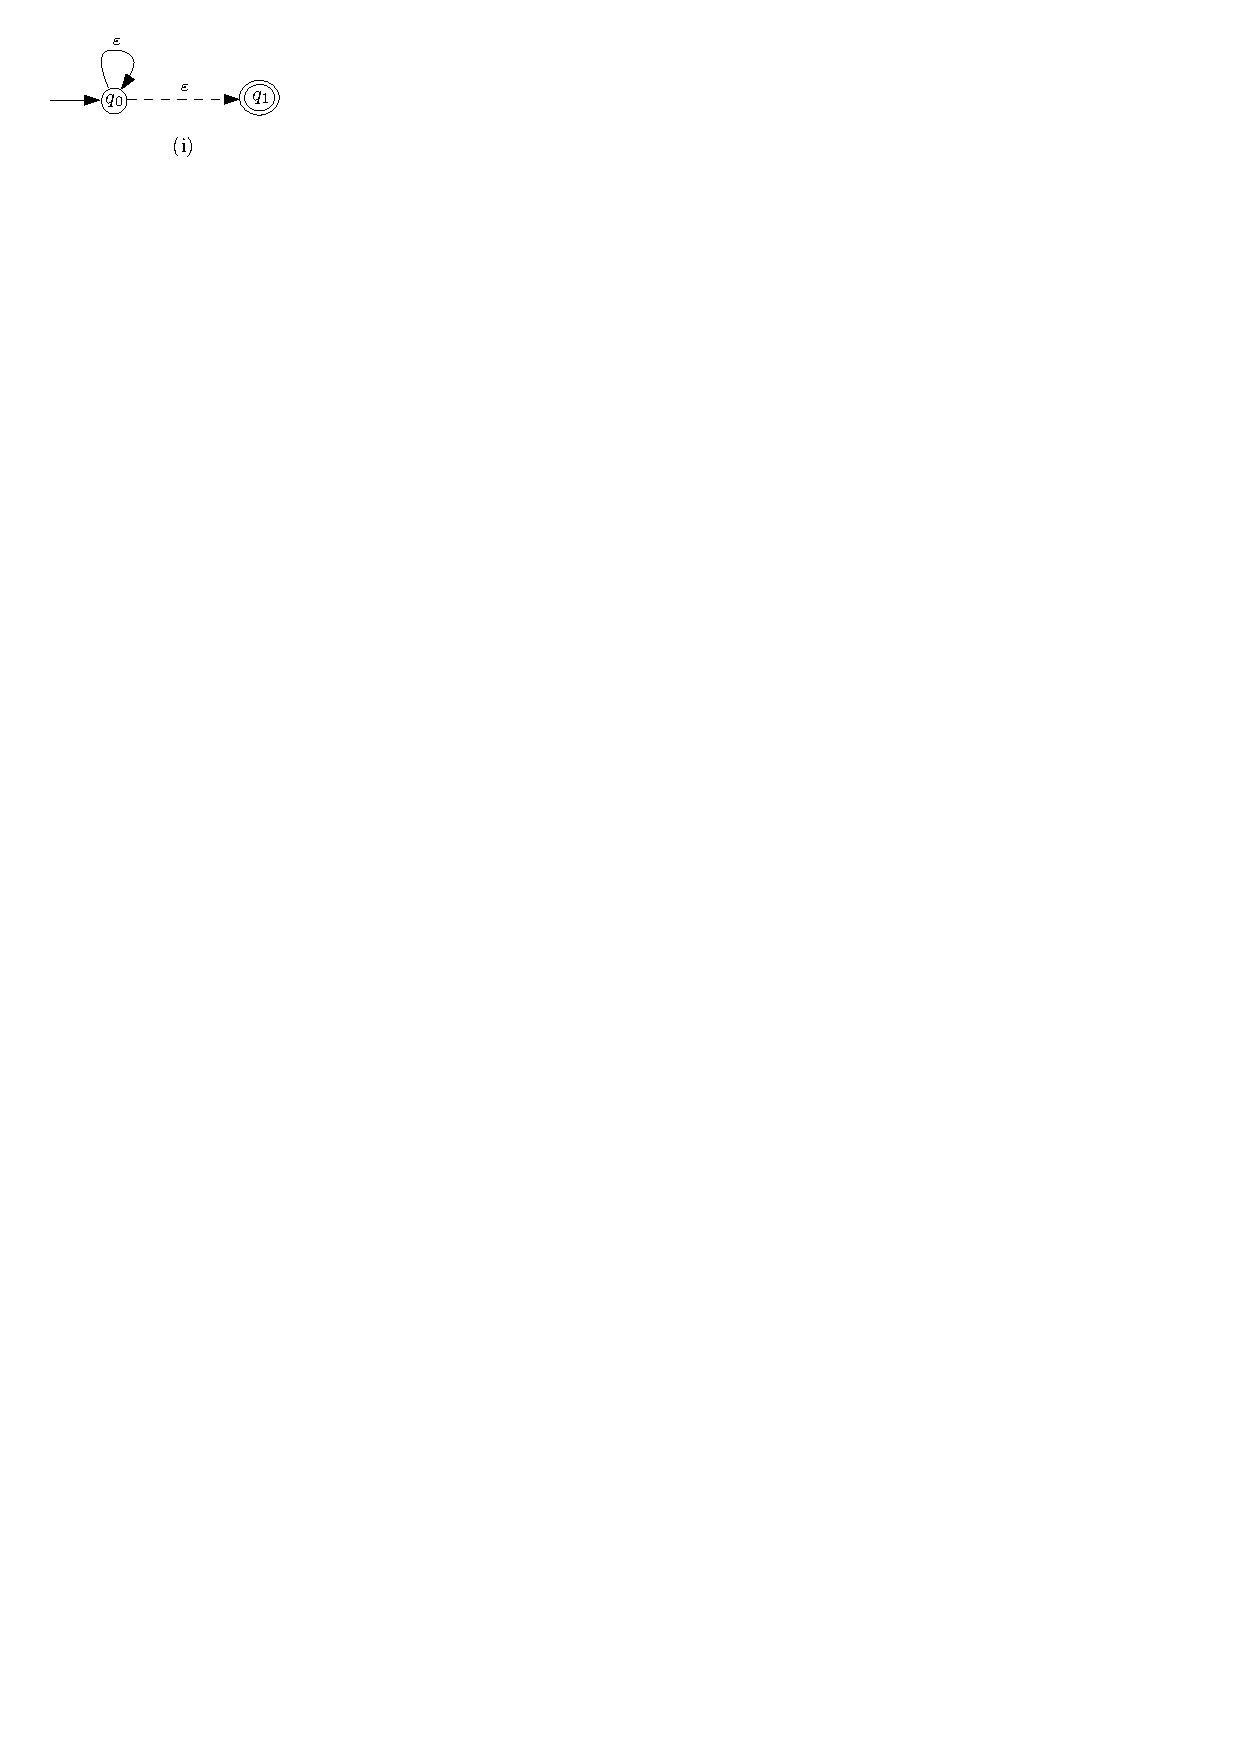
\includegraphics[scale=0.8]{pfa-epsilon-star.pdf}
%\caption{The PFA for $\varepsilon^\ast$}
%\label{fig-pfa-epsilon-star}
%\end{figure}


\vspace{-1mm}
\begin{example}\label{exmp-pfa}
The PFA corresponding to the RWRE $e = [[([\Gamma^+])\concat .?] \concat ([\Gamma^*])]$ in Example~\ref{exmp-regex-match-tree} is illustrated in Fig.~\ref{fig-pfa}, where the dashed (resp. thicker solid) lines represent the $\varepsilon$-transitions of lower (resp. higher) priorities than non-$\varepsilon$ transitions (if there is any), and the doubly circled states are final states. For instance, $\delta(q_1, \ell) = (q_1)$ for every $\ell \in \{0, \dots, 9\}$, $\delta(q_1, .) = ()$, $\tau(q_1) = ((); (q_2))$. Since the $\varepsilon$-transition has lower priority than the $\ell$-transition at the state $q_1$, whenever the currently scanned letter is $\ell \in \{0,\cdots,9\}$ at $q_1$,  the PFA will choose to go to $q_1$ greedily, until there is no more $\ell  \in \{0,\cdots,9\}$. (In this case, it has to choose the $\epsilon$-transition and goes to $q_2$.)
%
\begin{figure}[ht]
\vspace{-2mm}
\centering
%\rule{\linewidth}{0cm}
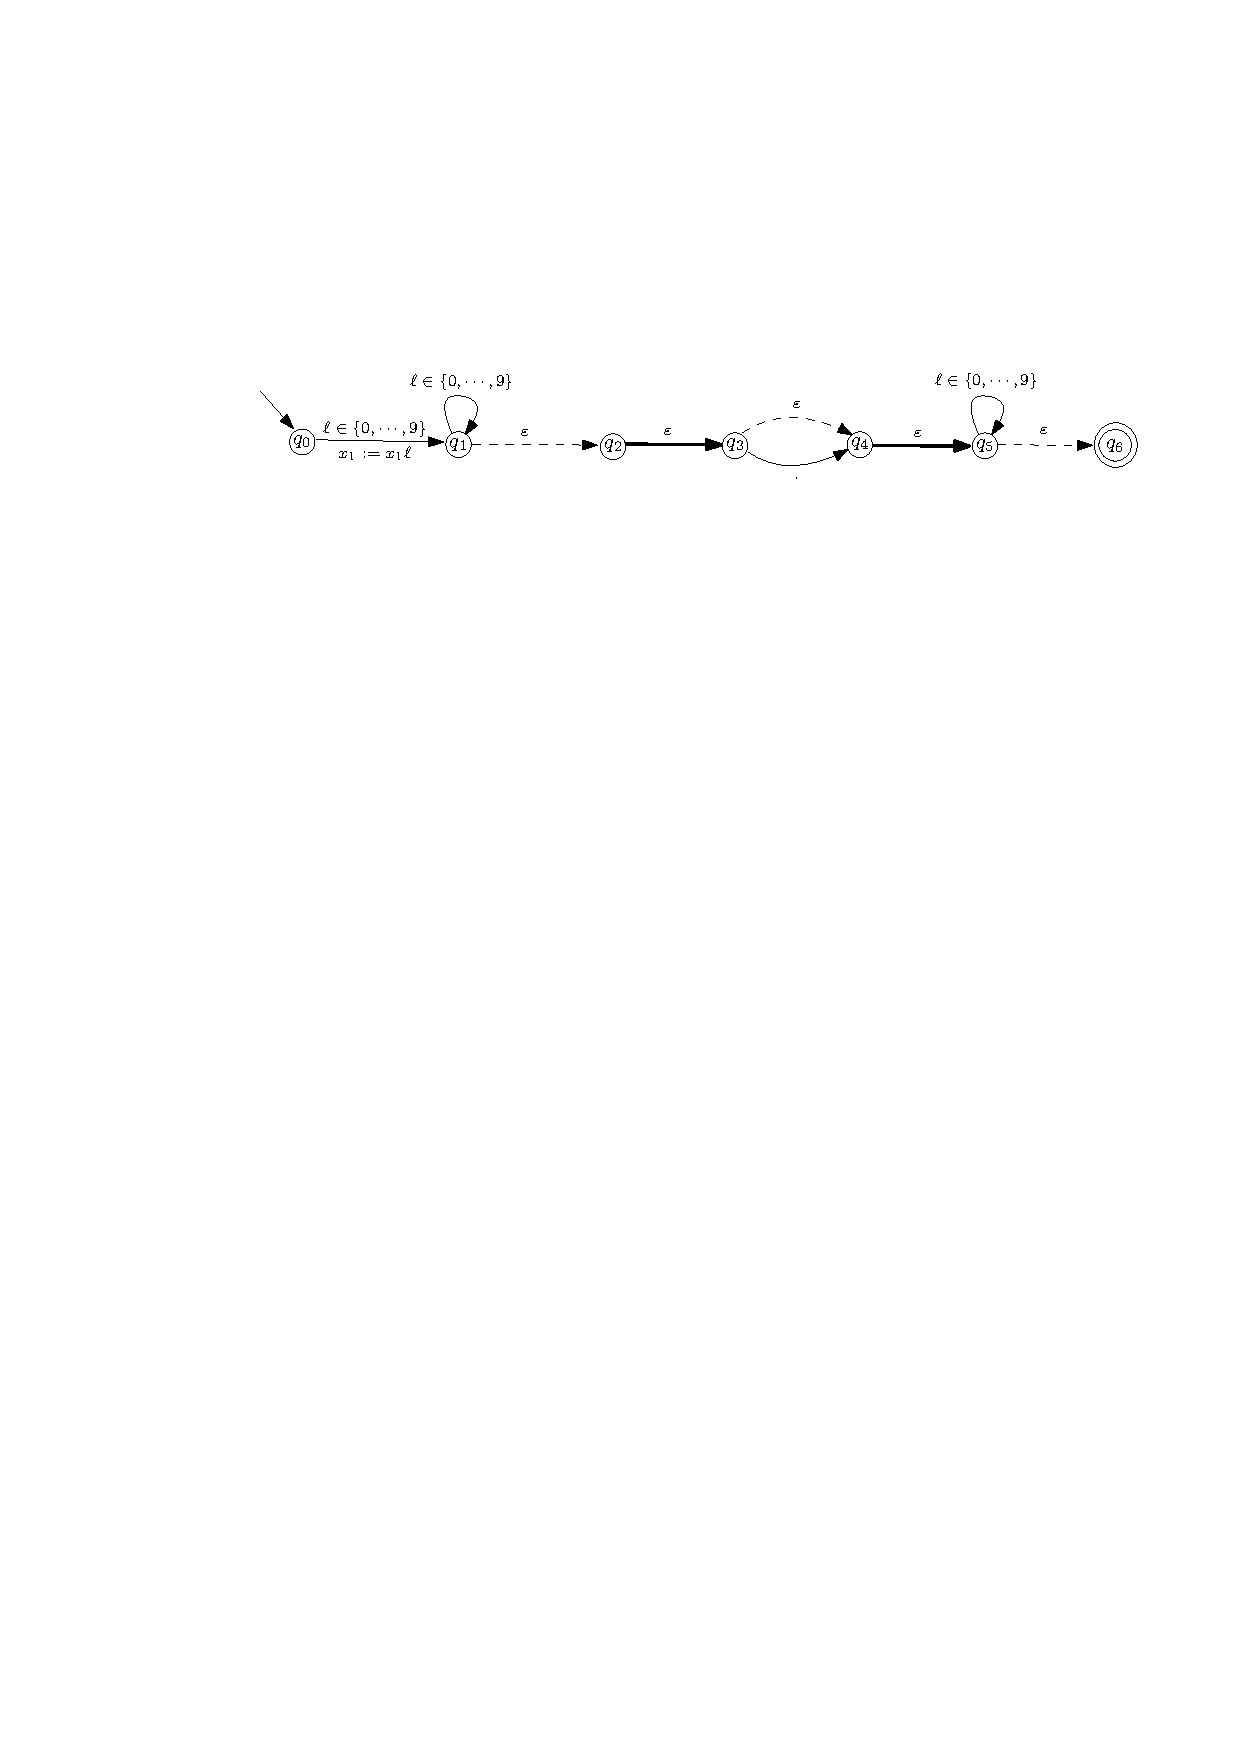
\includegraphics[width=0.9\textwidth]{pfa-new.pdf}
\caption{The PFA for $e = [[([\Gamma^+])\concat .?] \concat ([\Gamma^*])]$, where $\Gamma = \{0, \cdots, 9\}$}
\label{fig-pfa}
\vspace{-4mm}
\end{figure}
\end{example}

%%%%%%%%% The old example for PFA %%%%%%%%%
\hide{
\begin{example}\label{exmp-pfa}
The PFAs corresponding to $a^\ast$ and $a^{\ast?}$ respectively are illustrated in Figure~\ref{fig-pfa}(i) and (ii), where the dashed line represents $\pi_2(\tau(q_0))$ (of lower priority than the $a$-transition), the thicker solid line represents $\pi_1(\tau(q_0))$ (of higher priority than the $a$-transition), and the doubly circled state $q_1$ is a final state.

\begin{figure}[ht]
\centering
%\rule{\linewidth}{0cm}
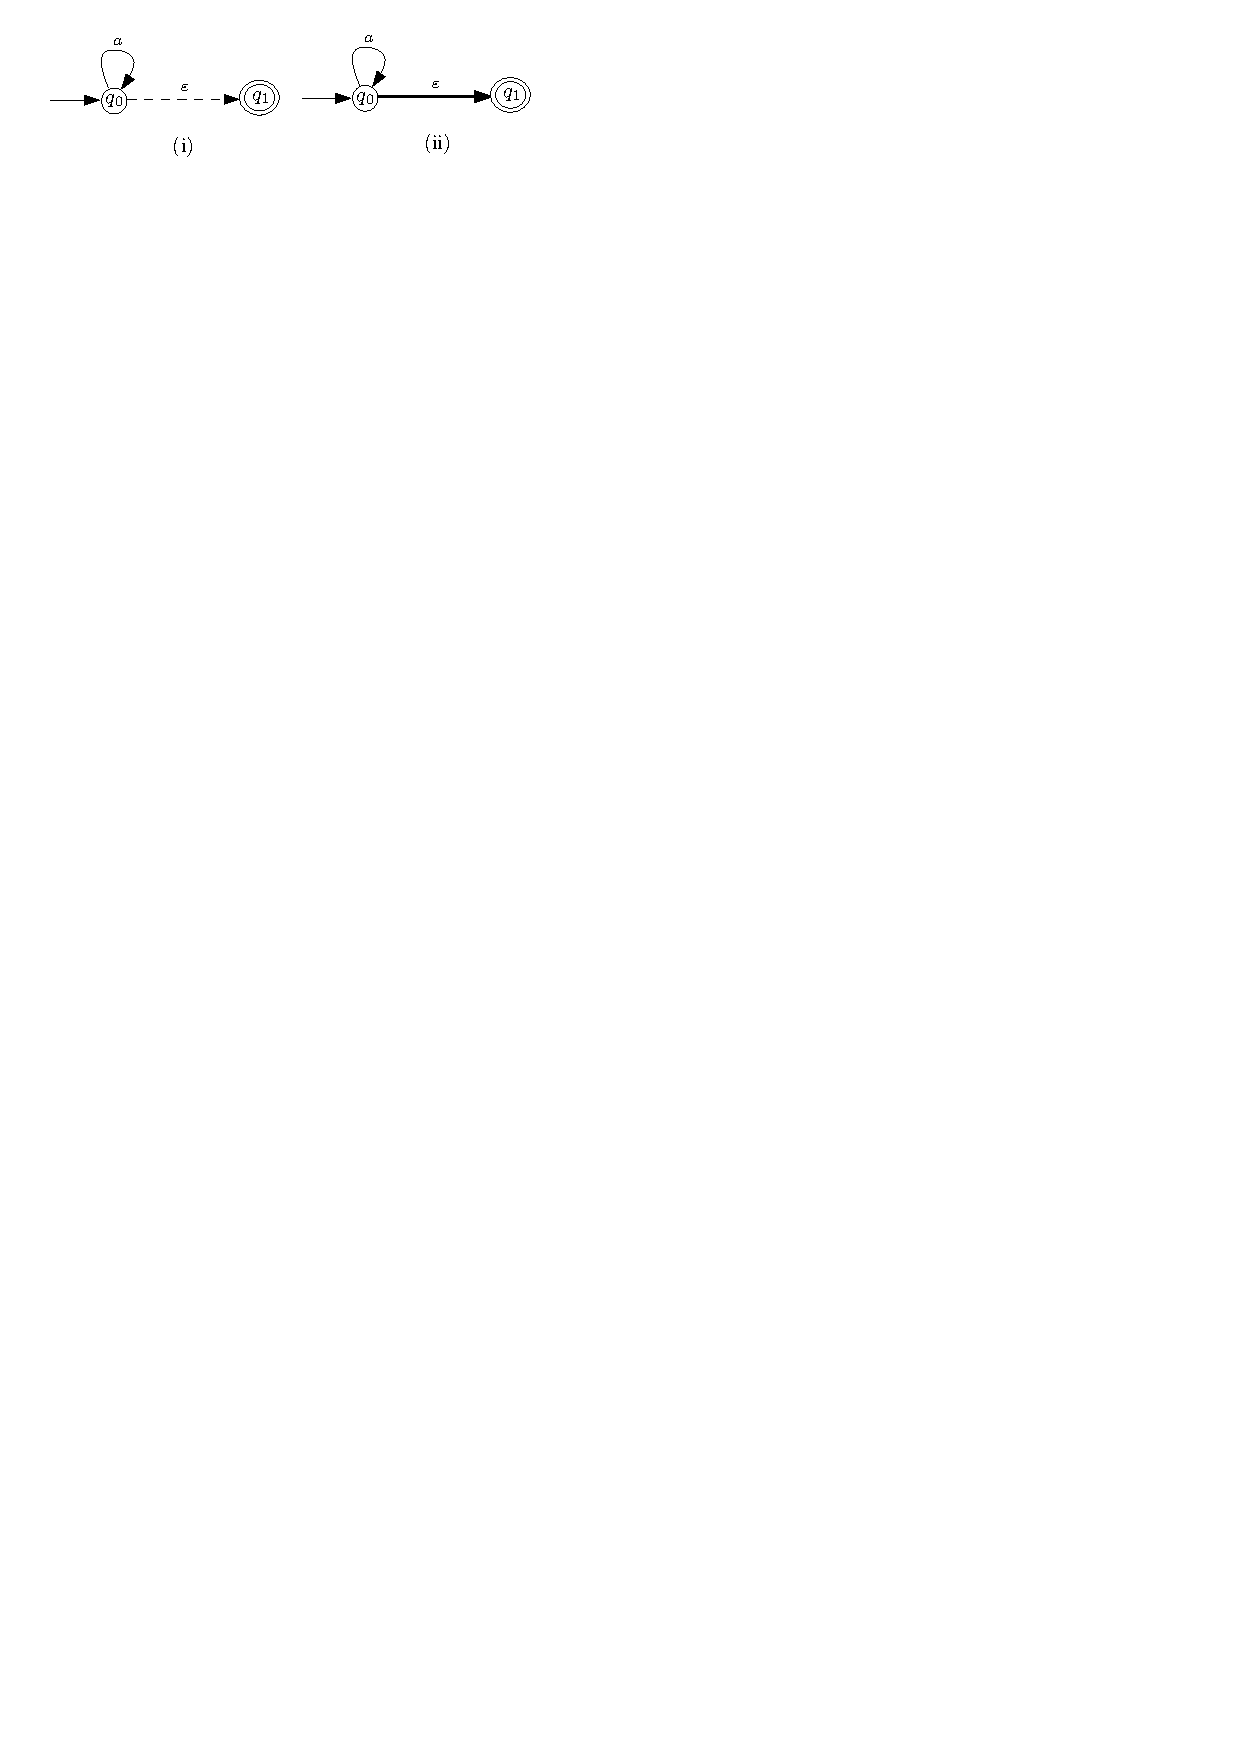
\includegraphics[width=0.6\textwidth]{pfa.pdf}
\caption{The PFAs for $a^\ast$ and $a^{\ast?}$}
\label{fig-pfa}
\end{figure}
\end{example}
}
%%%%%%%%% The old example %%%%%%%%%

%\begin{remark}
%Remark that PFAs in Definition~\ref{def-pfa} are different from pNFAs in \cite{BM17} in the sense that the state set in a pNFA is partitioned into two disjoint subsets and the non-$\varepsilon$-transitions are deterministic, while this is not the case in PFAs. Therefore, PFAs are slightly more flexible than pNFAs in \cite{BM17}. We choose this definition of PFAs as a more natural extension of FAs. 
%\end{remark}

%The priorities of PFAs are used to model the greedy and non-greedy semantics of $\regexp$. %, as we shall see in Section~\ref{construction:pnfa}.
%
%\paragraph{Prioritized streaming string transducers.}
%

We are ready to define prioritized streaming string transducers. 
%a new class of transducers that combine prioritized finite-state automata \cite{BM17} %which combines the expressive power of 
%and streaming string transducers \cite{AC10,AD11}.
  
\vspace{-2mm}  
\begin{definition}[Prioritized Streaming String Transducers]
A \emph{prioritized streaming string transducer} (PSST) is a tuple $\psst = (Q, \Sigma, X, \delta, \tau, E, q_0, F)$, where $Q$ is a
finite set of states, $\Sigma$ is the input and output alphabet such that $\nullchar \not \in \Sigma$, $X$ is a finite set of variables, $\delta \in Q \times \Sigma \rightarrow \overline{Q}$, $\tau \in Q \rightarrow \overline{Q} \times \overline{Q}$, $E$ is a partial function from $Q \times \Sigma^\varepsilon \times
  Q$ to $X \rightarrow \{\nullchar\} \cup (X \cup \Sigma)^{\ast}$, i.e. the set of assignments,
   $q_0 \in Q$ is the initial state, and $F$ is a partial function
  from $Q$ to $(X \cup \Sigma)^{\ast}$.
\end{definition}
\vspace{-1mm}
In the definition of PSSTs, the special symbol $\nullchar$ is introduced to capture the situation that $\extract_{i,e}(x)$ returns $\nullchar$, i.e. $x \in \Lang(e)$ but the $i$-th capturing group of $e$ is not matched.

A run of $\psst$ on a string $w$ is a sequence $q_0 a_1 s_1 q_1 \ldots a_m s_m q_m$ such that
\begin{itemize}
%\item $q_m \in F$,
%
\item for each $i \in [m]$, 
\begin{itemize}
\item either $a_i \in \Sigma$, $q_i \in \delta (q_{i-1}, a_i)$, and $s_i = E (q_{i - 1}, a_i, q_i)$, 
\item or $a_i = \varepsilon$, $q_i \in \tau(q_{i-1})$ and $s_i = E (q_{i - 1}, \varepsilon, q_i)$,
\end{itemize}

%\item for every subsequence $q_i a_{i+1} s_{i+1} q_{i+1} \ldots a_{j} s_j q_j$ such that  $i < j$ and $a_{i+1} = \cdots = a_j = \varepsilon$, it holds that $q_i, \ldots, q_j$ are mutually distinct. (Intuitively, loops of $\varepsilon$-transitions are forbidden.) 
\item for every subsequence $q_i a_{i+1} s_{i+1} q_{i+1} \ldots a_{j} s_j q_j$ such that  $i < j$ and $a_{i+1} = \cdots = a_j = \varepsilon$,  it holds that for every $k, l: i \le k < l < j$, $(q_k, q_{k+1}) \neq (q_l, q_{l+1})$.
\end{itemize}

%A run of $\psst$ is the sequence $q_0 a_1 s_1 q_1 \ldots a_m s_m q_m$, where $F (q_m)$ is defined and for each $i \in [m], q_i \in \delta (q_{i-1}, a_i)$ and $s_i = E (q_{i - 1}, a_i, q_i)$. 
For any pair of runs $R = q_0 a_1 s_1 \ldots a_m s_m q_m$ and $R' = q_0 a'_1
  s_1' \ldots a'_n s_n' q_n'$ such that $a_1 \ldots a_m = a'_1 \ldots a'_n$, the definition that $R$ is of a higher priority over
  $R'$ is similar to PFAs.
  % $p \neq p'$ and, for the smallest index $j$ with $q_j \neq q_j'$,
 % $\delta (q_{j - 1}, a_j) = \ldots q_j \ldots q_j' \ldots$
  
An accepting run of $\psst$ on $w$ is a run of $\psst$ on $w$, say $R = q_0 a_1 s_1 \ldots a_m s_m q_m$, such that 1) $F(q_m)$ is defined, 2)  $R$ is of the highest priority among those runs satisfying 1). The output of $\psst$ on $w$, denoted by $\psst(w)$, is defined as $\eta_m(F(q_m))$, where $\eta_0(x) = \varepsilon$ for each $x \in X$, and $\eta_{i}(x) = \eta_{i-1}(s_{i}(x))$ for every $1 \le i \le m$ and $x \in X$. Note that here we abuse the notation $\eta_m(F(q_m))$ and $\eta_{i-1}(s_{i}(x))$ by taking a function $\eta$ from $X$ to $(\Sigma \cup \{\nullchar\} )^*$ as a function from $(X \cup \Sigma \cup \{\nullchar\})^*$ to $(\Sigma \cup \{\nullchar\})^*$, which maps each $x \in X$ to $\eta(x)$, each $a \in \Sigma$ to $a$, and $\nullchar$ to $\nullchar$ . If there is no accepting run of $\psst$ on $w$, then $\psst(w) = \bot$, that is, the output of $\psst$ on $w$ is undefined. The string relation defined by $\psst$, denoted by $\cR_\psst$,  is 
$$\{(w, \psst(w)) \mid w \in \Sigma^\ast, \psst(w)  \in \Sigma^* \cup \{\nullchar\}\}.$$
Note that in the definition of $\cR_\psst$ above, the inputs of $\psst$ whose outputs are in $(\Sigma \cup \{\nullchar\})^* \setminus (\Sigma^* \cup \{\nullchar\})$ are ignored.

\vspace{-1mm}
\begin{example}
The PSST $\cT_{\tt extract_{decimalReg,1}}=(Q, \Sigma, X, \delta, \tau, E,  q_{0}, F)$ mentioned in Section~\ref{sec:mot} is obtained from the PFA in Fig.~\ref{fig-pfa} by adding $x_1 := x_1 \ell$ to each $\ell$-transition going into $q_1$ (see Fig.~\ref{fig-psst-exmp}). More specifically, in $\cT_{\tt extract_{decimalReg,1}}$, we have $\Sigma = \{0,\cdots,9, .\}$, $X= \{x_1\}$ with $x_1$ recording the matches of the 1st capturing group, $F(q_{6}) = x_1$ denotes the final output, and $\delta, \tau, E$ are illustrated by the edges in Fig.~\ref{fig-psst-exmp}, where the dashed/ticker solid edges denote the $\varepsilon$-transitions of lower/higher priorities than the non-$\varepsilon$-transitions and the symbol $\ell$ is used to denote the currently scanned input letter. Note that the identity assignments, e.g. $E(q_3, ., q_4)(x_1) = x_1$, are omitted in Fig.~\ref{fig-psst-exmp}, for readability.   

%From $\delta(q_4, \backslash s) = q_5q_{6}$, we know that $q_5$ is prior to $q_6$. 
%Therefore, whenever $\cT_{\sf nameReg}$ reads $\backslash$s at the state $q_3$,  it will choose to go the state $q_5$ greedily, unless this choice would lead to the nonacceptance (in this case, $q_6$ will be chosen). 

\begin{figure*}[ht]
\vspace{-2mm}
\centering
%\rule{\linewidth}{0cm}
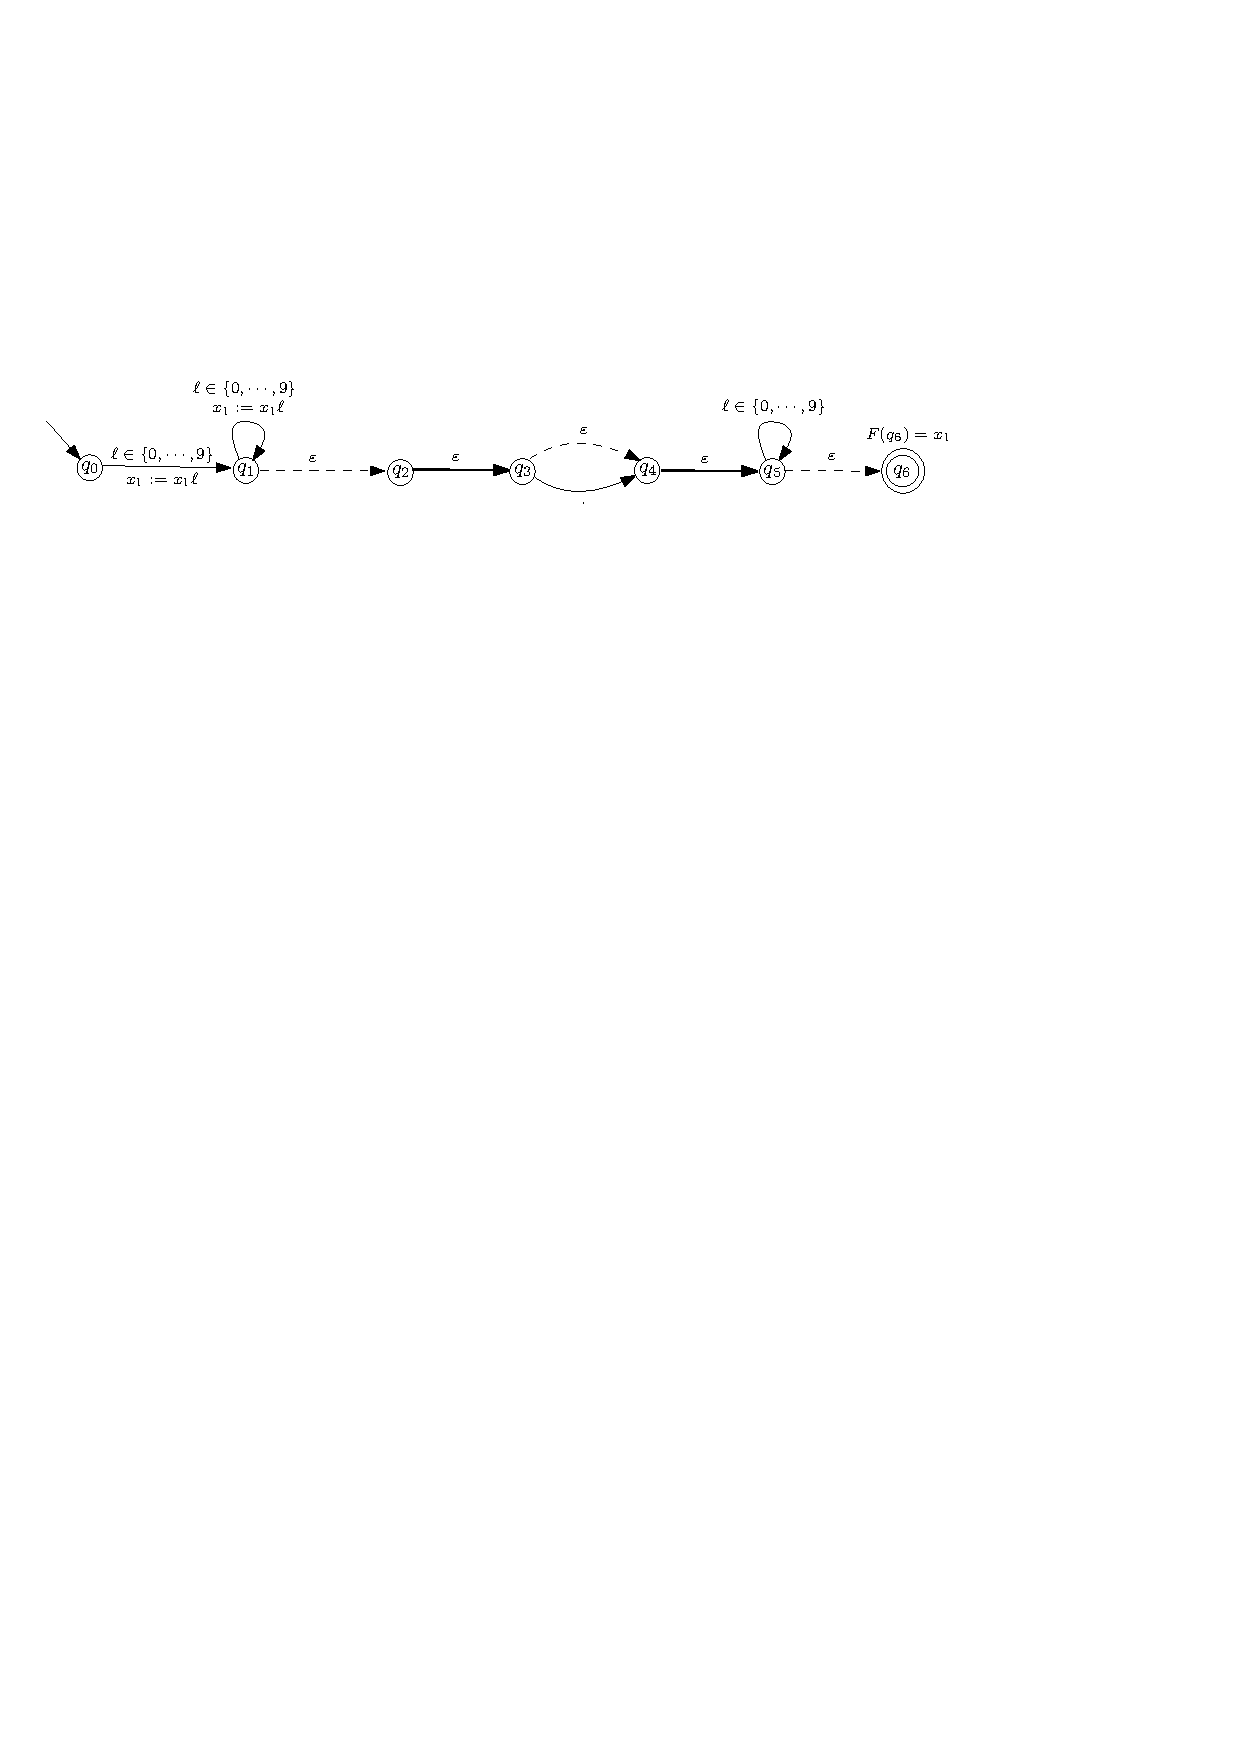
\includegraphics[width=0.95\textwidth]{psst-epsilon-exmp-new.pdf}
\caption{The PSST $\cT_{\tt extract_{decimalReg,1}}$}
\label{fig-psst-exmp}
\vspace{-3mm}
\end{figure*}
\end{example}

  
%  $\tmop{Out} (r) =
%  s_{\varepsilon} \circ s_1 \circ s_2 \ldots s_n \circ F (q_n)$ where
%  $s_{\varepsilon}$ is the empty substitution which maps all variables to
%  $\varepsilon$.
  

% Note that in the definition of \NSST, there is no \emph{copyless} restriction.



